\documentclass[a4paper]{article}
\usepackage[utf8]{inputenc}
\usepackage[czech]{babel}
\usepackage[margin=13mm, tmargin=15mm, bmargin=12mm]{geometry}
\usepackage{multirow}
\usepackage{tikz}
\usetikzlibrary{calc}
\usepackage{chngpage}
\usepackage{tabularx}
\usepackage{fancyhdr}
\usepackage{mathptmx}
\usepackage{lipsum}
\usepackage{float}

\renewcommand{\baselinestretch}{1.15}
\pagenumbering{gobble}
\pagestyle{fancy}
\renewcommand{\headrulewidth}{0pt}

\newcommand{\jmeno}{David Škrob}
\newcommand{\trida}{L4A}
\newcommand{\poradovecislo}{}
\newcommand{\nazevulohy}{Diody na RC2000}
\newcommand{\cisloulohy}{}
\newcommand{\predmet}{Technické měření}
\newcommand{\skupina}{}
\newcommand{\datummereni}{9.1.2023}
\newcommand{\datumodevzdani}{11.1.2023}
\newcommand{\klasifikace}{}

\begin{document}
\fancyhead{
\begin{tikzpicture} [overlay,remember picture]
       \draw
        ($ (current page.north west) + (1cm, -12mm) $)
        rectangle
        ($ (current page.south east) + (-1cm,12mm) $);
\end{tikzpicture}
}

\renewcommand{\arraystretch}{2}
\shorthandoff{-}

{
\begin{adjustwidth}[]{-3mm}{-3mm}
\centering
\vspace*{-7mm}
\begin{tabularx}{\linewidth}{l|X|p{3cm}}
\multirow{2}{25mm}{\centering SPŠ a VOŠ technická Brno, Sokolská 1} &
\textbf{LABORATORNÍ CVIČENÍ Z ELEKTROTECHNIKY} & Třída: \trida \\
\cline{2-3}
 & Jméno a příjmení: \jmeno & Poř. Číslo: \poradovecislo \\
\hline
\end{tabularx}

\begin{tabularx}{\linewidth}{X|p{3cm}}
Název úlohy: \nazevulohy & Číslo úlohy: \cisloulohy \\
\hline
Zkoušený předmět: \predmet & Skupina: \skupina \\
\hline
\end{tabularx}

\begin{tabularx}{\linewidth}{X|X|X}
Datum měření: \datummereni &  Datum odevzdání: \datumodevzdani &  Klasifikace: \klasifikace \\
\hline
\end{tabularx}

\end{adjustwidth}
}

\shorthandon{-}

\section*{Zadání}
Změřte voltamperové charakteristiky (VA), použijte modul V-A Characteristics. Voltampérové
charakteristiky v každém úkolu změřte do jednoho grafu.
\begin{figure}[h]
	\centering
	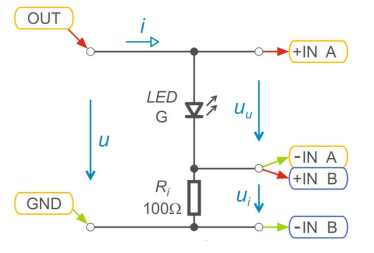
\includegraphics[width=0.4\textwidth]{zapojeni1.png}
	\caption{Schéma zapojení pro úlohy 1 - 5}
	\label{fig:schema15}
\end{figure}
\section*{Vypracování}
\begin{enumerate}
	\item VA usměrňovací diody a schottkyho diody a transilu
	\begin{figure}[H]
		\centering
		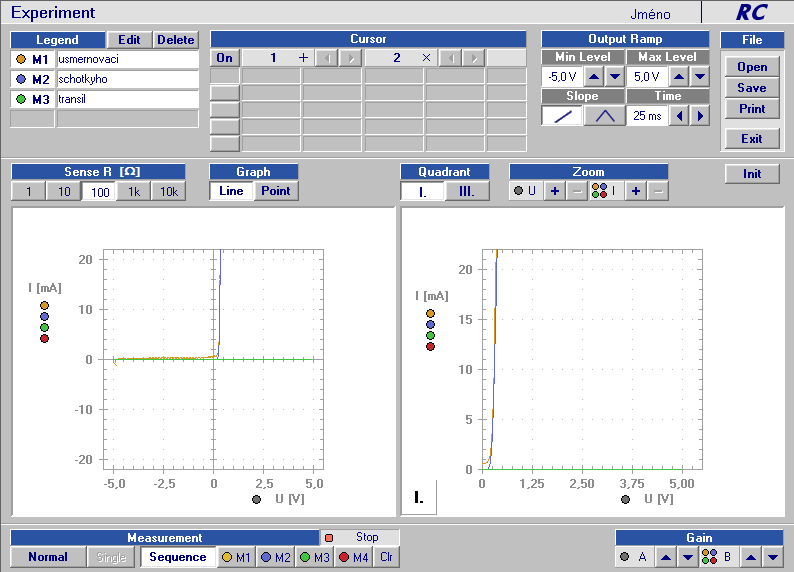
\includegraphics[width=0.75\textwidth]{9leden/diody1.png}
		\caption{Graf}
		\label{fig:mesh1}
	\end{figure}
	\item VA 4x LED (červena, zelená, žlutá, modrá)
	\begin{figure}[H]
		\centering
		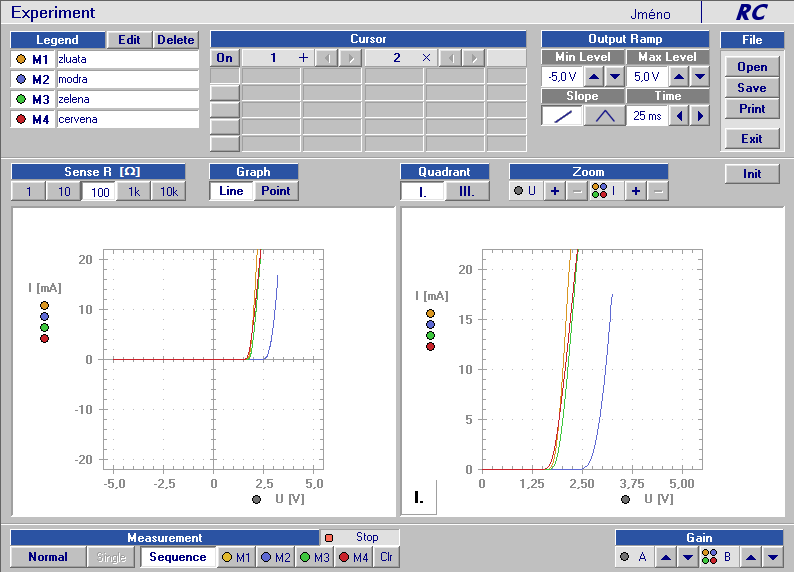
\includegraphics[width=0.75\textwidth]{9leden/ledky.png}
		\caption{Graf }
		\label{fig:mesh2}
	\end{figure}
	\item VA zenerovy diody pro napětí  2,4 V; 3,0 V; 3,6 V; 4,3 V
	\begin{figure}[H]
		\centering
		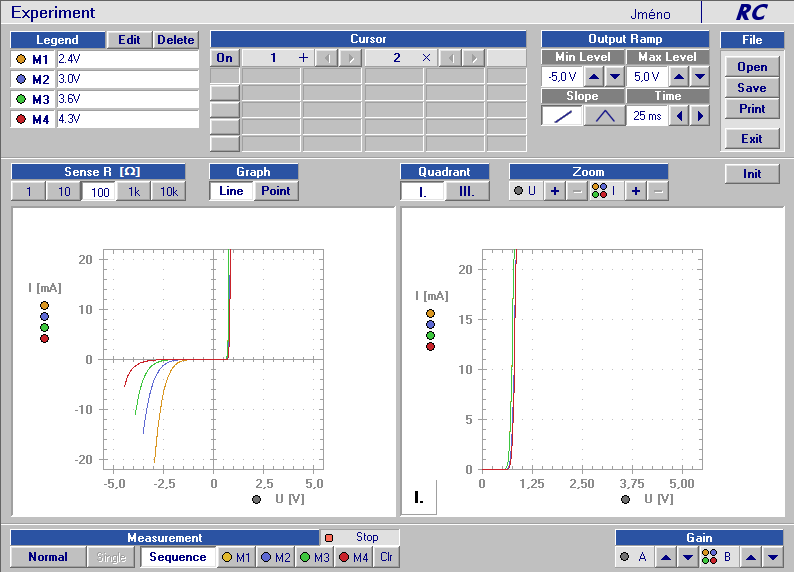
\includegraphics[width=0.75\textwidth]{9leden/zenerovy.png}
		\caption{Graf}
		\label{fig:mesh3}
	\end{figure}
	\item NTC rezistor při normální teplotě a zahřátý v prstech (cca 30 $s$)
	\begin{figure}[H]
		\centering
		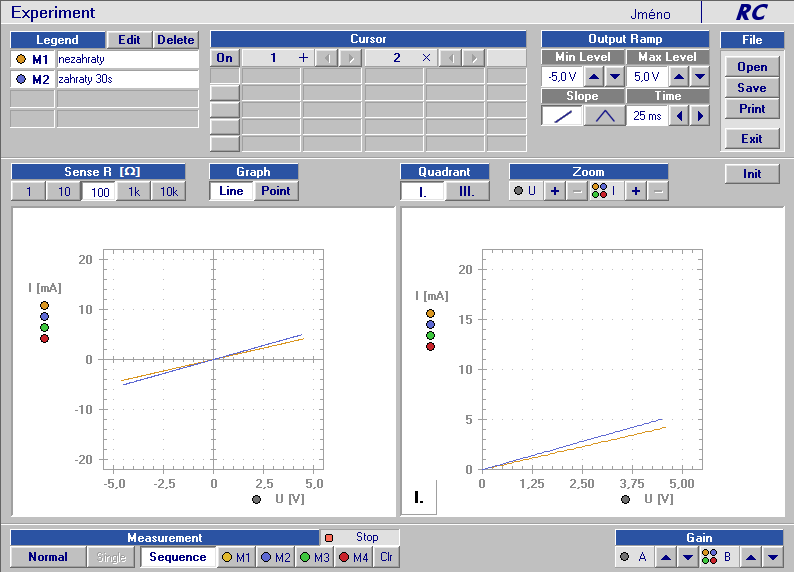
\includegraphics[width=0.75\textwidth]{9leden/NTCrezistor.png}
		\caption{Graf}
		\label{fig:mesh5}
	\end{figure}
	\begin{figure}[H]
		\centering
		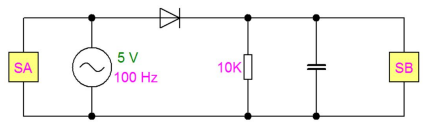
\includegraphics[width=0.5\textwidth]{zapojeni2.png}
		\caption{Schéma zapojení pro úlohu 6}
		\label{fig:mesh6}
	\end{figure}
	\item\begin{enumerate}
		\item Napětí na střídavém zdroji (sonda A)
		\item Napětí na rezistoru připojeném k diodě zapojené jako jednocestný usměrňovač (sonda B)
		\item Totéž jako v úkolu 6b + přidaný filtrační kondenzátor 1 $\mu F$, 2 $\mu F$, 5 $\mu F$
	\end{enumerate}
	\begin{figure}[H]
		\centering
		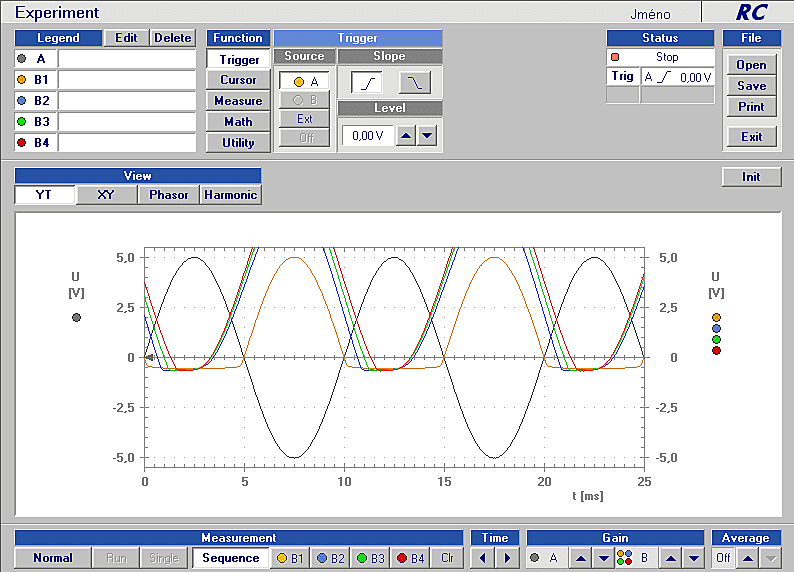
\includegraphics[width=0.75\textwidth]{6..png}
		\caption{vypracovani ukolu 6}
		\label{fig:mesh7}
	\end{figure}
	\begin{figure}[H]
		\centering
		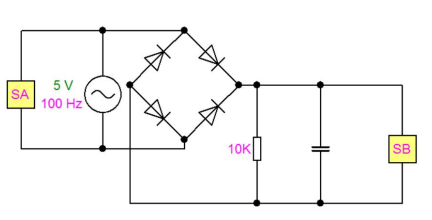
\includegraphics[width=0.4\textwidth]{zapojeni3.png}
		\caption{Schéma zapojení pro úlohu 7}
		\label{fig:mesh8}
	\end{figure}
	\item\begin{enumerate}
		\item Napětí na střídavém zdroji (sonda A)
		\item napětí na rezistoru připojeném ke dvoucestnému usměrňovači zapojenému ze 4 diod (Gr\"{a}tzovo
		zapojení)
		\item totéž jako v úkolu 7b + přidaný filtrační kondenzátor 1 $\mu F$, 2 $\mu F$, 5 $\mu F$
	\end{enumerate}
	\begin{figure}[H]
		\centering
		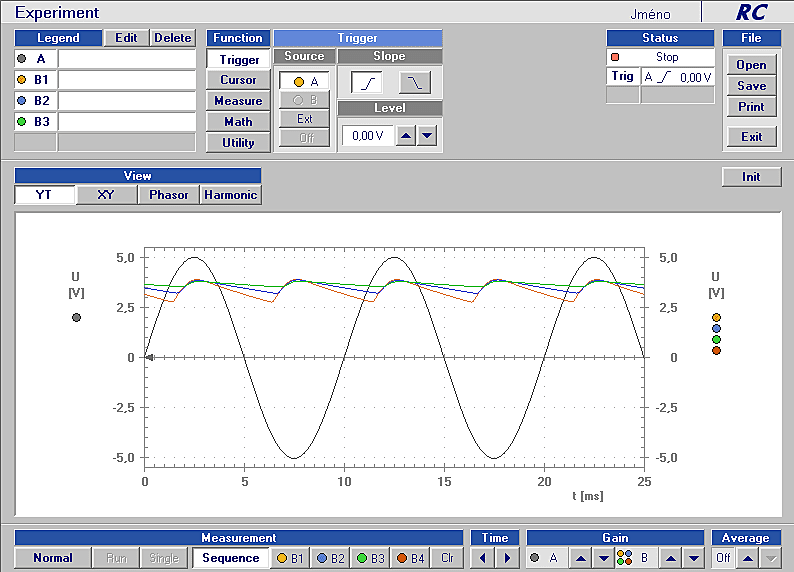
\includegraphics[width=0.75\textwidth]{7..png}
		\caption{vypracovani ukolu 7}
		\label{fig:mesh9}
	\end{figure}
\end{enumerate}


\section*{Závěr}
Data která jsem naměřil na RLC 2000, mě po předchozích laboratorních pracích a výkladu o diodách v technické fyzice v minulém ročníku nepřekvapil, avšak bylo přínosné vidět jak diody chovají v reálném světě. %Boužel jsme data z prvních 4 měření uložili v formátu \texttt{.va} takže jsme z uložených dat nebyli schopni vytvořit obrázky, které bychom mohli přiložit do protokolu.

\section*{Použité pomucky:}
\begin{list}{}{}
	\item \Large{RLC 2000}
\end{list}
\end{document}